\section*{Introduction}

\subsection*{General Research Importance AM}
Additive Manufacturing (AM) has the ability to produce more complex products than conventional manufacturing processes. Dimensional accuracy, repeatability and short production time are however challenging to achieve within AM processes. Specifically, extrusion based additive manufacturing processes for soft materials. If the prescribed problems could be overcome AM could replace these conventional methods for mass production and safe money due to its free form capabilities. 

\subsection*{Types of soft material processes}
Soft material extrusion based processes (SME) are typically divided into material jetting and material extrusion. The former is an AM process that uses drop-on-demand technology where the nozzle dispenses droplets of photo-polymer, layer by layer. The latter is referring to the process where a thermoplastic filament is extruded through a heated nozzle onto the build platform. The material solidifies as it cools.

\subsection*{Direct vs Indirect Geometry control}
Dimensional accuracy could be improved through the implementation of a real-time deposition geometry controller. Control of parameters influencing geometry indirectly, such as, ???? are described in ???? and is applied to both laser-based as well as SME processes. Direct geometry control has been performed for a laser-based AM process ???? using a laser-camera triangulation based vision (LCTV) system for geometry measurement. Recent work ???? describes the application of a LCTV system for SME processes. Work on the usage of a LCTV system for direct geometry control is currently limited. 

\subsection*{Algorithm design for detection}
Algorithms used for geometry detection from images generated by a LCTV system can be divided into image segmentation, laser line extraction and feature extraction as described in \cite{li2007recent}.

\subsubsection*{Image segmentation}
The goal of image segmentation is to divide the image into separate sections to find important regions-of-interest (ROI) and improve computational efficiency. 

% ROI
Manual selection of region size and position as in \cite{huang2012development} is only effective for detection of static positioned objects. Another paper \cite{wang2014weld} manually selects ROI size while position is determined by the peak average column intensity of the image in gray-scale. This allows for deposition movement with constant region size. An algorithm to find the ROI position in both directions and determine the size automatically is described in \cite{xu2004features} where manual thresholding is used to separate back- and foreground. The bounding box is determined by the maximum and minimum positions of the pixels left after thresholding. 

% Laser line segmentation
Laser line segmentation is often achieved through thresholding methods. Global thresholding is used in \cite{zhang2007vision} where the thresholding value is determined by inspection of the image histogram. In \cite{wang2014weld} the threshold value is automatically determined by using the average of the maximum and minimum pixel intensity. A commonly used histogram thresholding method based upon maximizing the variance between the back and foreground is Otsu's method \cite{otsu1979threshold}. Also entropy based methods exist such as in \cite{liu2006image}.

\subsubsection*{Laser line extraction}
Line extraction is used to convert the laser line segment to a pixel position vector representing deposition geometry. 

% Fore- and background segmentation
A common method  \cite{nguyen2014laser} \cite{kim1995robust} \cite{li2010measurement} \cite{huang2012development} is to use peak pixel intensity value of the gray-scale image of each column or row as the laser line position. Others \cite{davis2011vision} \cite{xu2004features} \cite{zhang2007vision} take the maximum pixel difference of the segment edges and set the middle as the laser position. There also exist methods based upon morphology and the watershed algorithm as described in \cite{li2007recent}.

% Noise filtering
Noise makes it often impossible to detect the laser position for a column or row accurately. To account for these inhomogeneities in the laser line interpolation in combination with an moving average filter can be used as described in \cite{wang2014weld}. The distinction between the laser line and background regions is often disturbed. Convolution based filtering with different kernel sizes and shapes are used in\cite{huang2012development} where a Gaussian shaped kernel of size $7x7$ is applied to smooth the image. In \cite{zhang2007vision} a median filter is used where each pixel value is replaced by the median of neighboring pixels. There are also frequency based filtering methods as applied in \cite{uzun2005fpga} and wavelet methods such as in \cite{liu2006image}. Next to filtering in the spatial domain there are also papers which filter in the temporal domain. Removing noise by taking the smallest intensity of each pixel from consecutive images is described in \cite{li2010measurement}.

\subsection*{Feature Extraction}
Extraction of geometric features is application specific. A common approach is to label certain point on the laser line as feature points. Dimensions can then be calculated by the difference between those points. The simplest methods \cite{li2010measurement} \cite{huang2012development} rely on taking second derivatives of the laser line and labeling the absolute values as feature points. In \cite{kim1995robust} the laser line is segmented into small sections connected to each other (feature points) using polygonal fitting. Paper \cite{davis2011vision} decides if a point is a feature point based upon linguistic rules set by a threshold. 

\subsection*{Problems with the algorithms}
Many algorithms depend on parameters which need to tuned specifically for each application.  Different deposition material properties such as reflectiveness or transparency is not accounted for. Noise and disturbance in hardware components is also often neglected. 

\subsection*{Project Goal}
The goal of this report is therefore to design a flexible and robust vision-based detection algorithm able to detect deposition height and width for SME processes. The algorithm should be able to function for different robust against changing operating conditions affecting hardware components


\section*{Materials}

\subsection*{Triangulation configuration}

\begin{figure}[!ht]
   \centering
   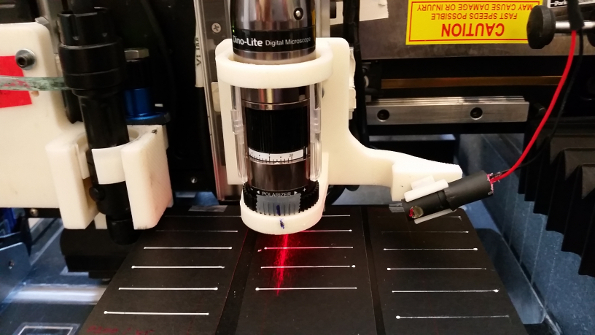
\includegraphics[width=0.40\textwidth]{setup_real.jpg}
   \setlength{\unitlength}{0.06\textwidth}
   \thicklines
   {\color{brown}\put(-7,3.3){\vector(3,-1){3.4}}}
   \footnotesize\put(-7.85,3.25){Camera}
   {\color{brown}\put(-7,2){\vector(3,-1){1.5}}}
   \footnotesize\put(-8,2){UV light}
   \footnotesize\put(-8,1.8){source}
   {\color{brown}\put(-7,0.6){\vector(1,0){3.3}}}
   \footnotesize\put(-8,0.55){Laser line}
   {\color{brown}\put(0.15,3.5){\vector(-3,-1){3.1}}}
   \footnotesize\put(0.2,3.45){Mount}
   {\color{brown}\put(0.15,2.2){\vector(-3,-1){1.65}}}
   \footnotesize\put(0.2,2.15){Laser}
   {\color{brown}\put(0.15,1.05){\vector(-3,-1){1.5}}}
   \footnotesize\put(0.2,1.00){Deposited}
   \footnotesize\put(0.2,0.8){material}
   \caption{Overview of vision system in reality.}
   \label{fig:setup_real}
\end{figure}

\subsection*{Camera}

\subsection*{Line Laser}

\subsection*{Deposition Material}


\chapter*{Methods}

\subsection*{Overview Algorithm}
With image segmentation

\subsection*{Deposition Segmentation}

\subsection*{Laser line edge segmentation}

\subsection*{Width Measurement}

\subsection*{Height Measurement}


\chapter*{Results}



\chapter*{Discussion}


